\documentclass{standalone}
\usepackage{chez}

\begin{document}
\chapter{December 07, 2020}

The next two days will be about the future,
i.e.\ what exists in algebraic topology outside of this class.
In this course, we focused on four topics:
\begin{itemize}[nosep]
  \item category theory
  \item homological algebra (\(\cchAb\), \(D(\ZZ)\), \(\Tor\), \(\Ext\))
  \item homotopy theory (study of \(\cHoTop\))
  \item algebraic topology (study of \(\cTop\), and in particular manifolds)
\end{itemize}

\section{Category theory}
We studied products and pushouts,
  which are special cases of \vocab{limits} and \vocab{colimits}.
We also studied curring isomorphisms,
  which are special cases of \vocab{adjunctions}.
Since the early 2000s, people also like to study
  \vocab{higher categories} or \vocab{\(\infty\)-categories}, where there are
\begin{enumerate}
  \item objects,
  \item morphisms,
  \item \(2\)-morphisms, or morphisms between morphisms,
\end{enumerate}
and these can keep going on.

\begin{example}
  \(H\ZZ\)-modules are the \(\infty\)-category of chain complexes, where
  \begin{itemize}
    \item objects are chain complex of abelian groups,
    \item morphisms are chain maps between complexes,
    \item \(2\)-morphisms are chain homotopies between chain maps.
  \end{itemize}
\end{example}

\begin{example}
  \(\mathcal S\) is the \(\infty\)-category of homotopy theory, where
  \begin{itemize}
    \item objects are topological spaces,
    \item morphisms are continuous maps, and
    \item \(2\)-morphisms are homotopies.
  \end{itemize}

  We can make an equivalent \(\infty\)-category with
  a combinatorial definition with simplicial sets.
\end{example}

\begin{example}
  \(\cat{Cat}_2\) is the \(\infty\)-category of categories, where
  \begin{itemize}
    \item objects are categories,
    \item morphisms are functors,
    \item \(2\)-morphisms are natural transformations.
  \end{itemize}
\end{example}

To learn more, Google \texttt{Kerodon}.


\section{Homological algebra}
Homological algebra a developed much more in algebraic geometry (i.e.\ 18.726).

In particular, there are things called sheaf \(\Hom\), sheaf \(\Ext\),
sheaf cohomology, etc.

\begin{adhoctheorem}{Idea}
  \(\set{x^2 + y^2 - 1 = 0} \subseteq \RR^2\) is an algebraic way
  of describing the circle.
  Can one come up with a purely algebraic algorithm for calculating,
  starting with a set of polynomials with real coefficients,
  the homology of the set of those solutions?

  What happens if one applies these algorithms to polynomials
  with coefficients in a number field?
\end{adhoctheorem}


\section{Homotopy theory}
This is ``the study of the equals sign'', or better yet,
``the study of the isomorphism sign''.

Suppose there is a CW-complex with two objects and a path.
This can be thought of as two object,
and the path between them tells us that \(a = b\).
In particular, we can identify the two objects,
and think of this as a single object.
\begin{center}
  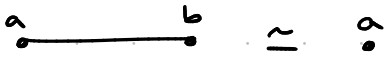
\includegraphics[width=0.25\textwidth]{18_905-201207-1.png}
\end{center}

On the other hand, if we have two objects with two paths between them,
i.e.\ they are equal in two different ways.
In particular, there are two different equalities between them.
We can use one path to identify them,
but then we have the other equality left.
This is the same as a single object with a nontrivial automorphism.
\begin{center}
  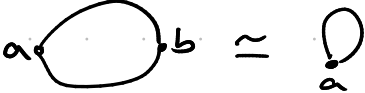
\includegraphics[width=0.25\textwidth]{18_905-201207-2.png}
\end{center}

Similarly, if we have an extra object
  \(c\) that is uniquely identified with \(b\),
  then we identify \(b\) and \(c\),
  and then it reduces to the previous case.
\begin{center}
  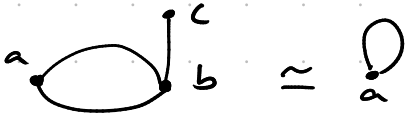
\includegraphics[width=0.25\textwidth]{18_905-201207-3.png}
\end{center}

Note that these are just homotopy equivalences of graphs.
In the spirit of higher category theory,
we can also think about equalities between equalities.
\begin{center}
  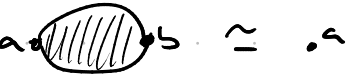
\includegraphics[width=0.25\textwidth]{18_905-201207-4.png}
\end{center}
This is equivalent to saying \(D^2 \simeq *\).

In general, homotopy theory is about objects, equalities between objects,
\(2\)-equalities between equalities, etc.


\section{Algebraic topology}
One example of a question we ask in algebraic topology is:
``Can we classify all \(n\)-dimensional compact manifolds up to homomorphism?
  What about smooth manifolds up to diffeomorphism?''

For example, surfaces (\(2\)-dimensional compact manifolds) are classified.
For example, \(\ZZ\)-oriented surfaces are classified by their genus.
In particular, it is determined by its first homology group.

However, when we increase the dimension, the manifolds get very complicated,
so we can ask the question about manifolds with particularly simple homology.
\begin{theorem}[Kervaire-Milnor, 1961]
  Classification of all compact simply connect \(n\)-dimensional
  manifolds \(M\) with
  \[
    H^q(M) \iso \begin{cases*}
      \ZZ & if \(q = 0, n\) \\[-1ex]
      0 & otherwise
    \end{cases*}
  \]
  for \(n \geq 5\).
  For lower dimensions, we have known \(n = 2\) since around 1900,
  we know \(n = 3\) due to Perelman in 2003, and \(n = 4\) is still unknown.
\end{theorem}

We can also ask if we can classify simply connected and compact
\(2n\)-dimensional manifolds \(M\) where \(H_0(M) \iso \ZZ\) and
\[
  H_1(M) \iso H_2(M) \iso \dots \iso H_{n - 1}(M) \iso 0.
\]
Every simply connected space is \(\ZZ\)-orientable, so it follows that
\[
  H_{n+1}(M) \iso H_{n+2}(M) \iso \dots \iso H_{2n}(M) \iso \ZZ.
\]
\(H_n(M)\) can be anything.
This is classified in all dimensions \(2n\) except \(2n = 4, 24, 126\).

\begin{itemize}
  \item \(n \equiv 6 \mod 8\) was proved by Wall in 1962
  \item \(n \equiv 5 \mod 8\) was proved by Brown and Peterson in 1966
  \item \(n \equiv 3 \mod 8\) was proved by Browder in 1969
  \item \(n \equiv 2 \mod 8\) was proved by Schultz in 1972
  \item \(n \equiv 1 \mod 8\) was proved by Stolz in 1985
  \item \(n \equiv 7 \mod 8\) and \(n \neq 63\) was done by
        Hill-Hopkins-Ravenel in 2009.
        At the time it was proved, Hopkins was a professor at MIT and
        Hill was a graduate student at MIT. % chktex 13
        He is now at UCLA and is the head of
        the LGBTQ society of mathematicians.
  \item \(n \equiv 0 \mod 4\) and \(n \neq 12\) was done by
        Burkland-Senger-Hahn in 2019. Burkland and Senger are
        grad students at MIT, and Hahn is the lecturer of this course!
        Adela Zhang is thinking about extending this to when
        two homology groups are nonzero.
\end{itemize}


\section{More homotopy theory}
\begin{question}
  If \(m\) and \(n\) are positive integers,
  how many maps are there from \(S^m \to S^n\) up to homotopy?
  The set of maps \(S^m \to S^n\) up to homotopy is denoted \(\pi_m S^n\).
\end{question}

On the homework, we proved \(\pi_3 S^2\) has more than one element.
In 18.906, we will see that
\begin{enumerate}
  \item If \(m < n\), all maps \(S^m \to S^n\) are homotopic,
        i.e.\ \(\pi_m S^n\) has one element.
  \item If \(m = n\), then \(\pi_m S^m \iso \ZZ\).
        Maps \(S^m \to S^m\) are determined up to homotopy by their degrees.
  \item If \(m > n\), then unless \(m = 2n - 1\), \(\pi_m S^n\) is finite.
\end{enumerate}
A natural question to ask is how large is this set?
Moreover, note that \(\pi_m S^n\) is not just a set,
but a group in the following way:
If we have two maps \(f, g \colon S^n \to S^n\),
we first ensure (by homotopy) that the south pole of \(f\)
is mapped to the same point as the north pole of \(g\).
Then, \(f * g\) is the map depicted in the following diagram,
where we first pinch the equator,
and then we map the top half by \(f\) and the bottom half by \(g\).
\begin{center}
  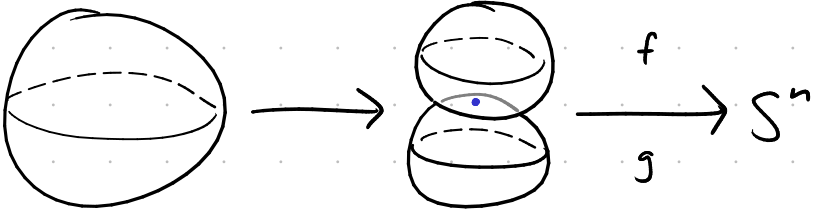
\includegraphics[width=0.5\textwidth]{18_905-201207-5.png}
\end{center}








\end{document}
